\documentclass[../report.tex]{subfiles}

\begin{document}

\chapter{Literature Review}

This section contains review of papers in bibliography. From these we take the foundation \& implement it for one example.

\section{Lagrangian Approach}
Consider the Dynamical System,
\begin{equation}
  \begin{aligned}
    \frac{d}{df}(n(t)) &= V((\frac{x}{t}), t) \\
    x_0 &= x(t_0) \\
    x \in \mathbb{R}^n &, t \in \mathbb{R}
  \end{aligned}
\end{equation}

For LCS, it is needed to compute Finite-Time-Lyapunov-Exponent (F.I.L.E), with a F.I.L.E for each grid point the structures can be plotted. \par

F.I.L.E is a scaler \(\sigma_{t_0}^T(n)\) which represents structures of a fluid at a location. The maximum show the atrocity (or repelling barriers). Let's say a particle at \(\mathcal{X}(t_0)\) goes to a new location after time \(T\). \par

Flow map of that point can be written as
\begin{equation}
  F_{t_0}^t(n_0) = n_0 + \int_{t_0}^{T} V(x(t), t)\,dt
\end{equation}

Let's say there is another point close to \(x(t_0)\) which is \(y = x + dx(t_0)\). After a time interval \(T\), distance between these 2 points becomes
\begin{equation}
  \begin{aligned}
    8n(t_0 + T) &= F_{t_0}^{toti} (y) - F_{t_0}^{toti} (x) \\
    &= \nabla F_{t_0}^{toti}(x)
  \end{aligned}
\end{equation}

From above equation we can calculate the neon strain tensor,
\begin{equation}
  \begin{aligned}
    C &= \nabla {F_{t_0}^{toti}(x)}^T \dot F_{t_0}^{toti}(n)
  \end{aligned}
\end{equation}

Eigan values of which are \(\lambda_1, \lambda_2, \dots, \lambda_n\) \& associated normalized eigenvectors, \(\epsilon_{\lambda_i}\;\; (i \in \{1, 2, 3, \dots, n\})\)

\(\therefore\) From the maximum eigenvalue of chuchy green tensor F.I.L.E can be calculated as
\begin{equation}
  \begin{aligned}
    \sigma_{t_0}^T (n_0) = \frac{1}{2|T|} \log(\lambda_n)
  \end{aligned}
\end{equation}

\#TODO: what?
\begin{equation}
  \begin{aligned}
    \lambda_n &= max\; eig (????) \\
    &= max\; eig(\nabla {F_{t_0}^{toti}(x)}^T \dot F_{t_0}^{toti}(n))
  \end{aligned}
\end{equation}

To complete F.I.L.E, it is necessary to have locations of particles at initial state \(t = t_0\) \& at \(t = t_0 + T\). \(\therefore\) Flow map can be determined.

\#TODO: Complete Formula
\begin{equation}
  \begin{aligned}
    {F_{t_0}^{toti}}^T &=
  \end{aligned}
\end{equation}
~ \\ ~ \\
\begin{figure}[H]
  \centering
  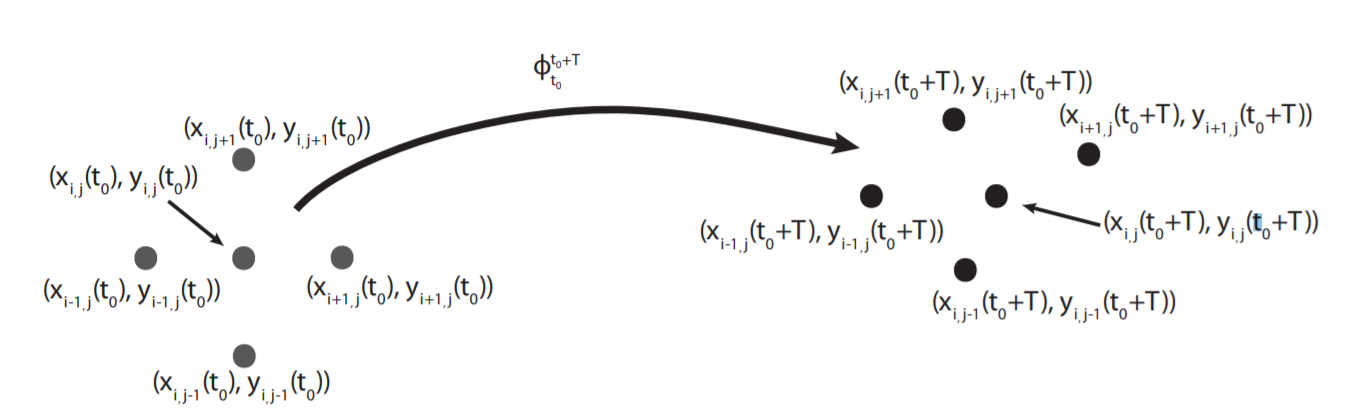
\includegraphics[width=0.8\linewidth]{images/image_1.png}
  \caption{\#TODO: Add Caption}
  \label{fig:fig-1}
\end{figure}

Now let's see the Eulerian Approach. \par

\section{Eulerian Approach}
The Eulerian role of strain Tensor is defined as
\begin{equation}
  \begin{aligned}
    S(n, t) = \frac{1}{2}{\nabla(x, t) + \nabla V(x, t)^T}
  \end{aligned}
\end{equation}
and eigan values of which are \(S_1 < S_2 < \dots < S_n\) and associated normalized eigen vectors, \(\epsilon_{S_i}\;\; i \in \{1, 2, \dots, n\}\) \par

From the eigen values of eulerian rate of stain tensor, one can identify regions of flow which are more attracting \& repelling. \par

There \(S_1\) \rightarrow minimum eigen values provides measure of attraction \& \(S_2\) maximum value of repulsion.

\subsection{Relation between Cauchy-Green Strain Tensor \& Eulerian Rate of Strain Tensor}
Eigen value of \(S\) as F.I.L.E limit as integration of time goes to 0. \par

For small \(|T|\), let us expand  \(C_{t_0}^t (n)\) as
\#TODO: Doubt in eq??
\begin{equation}
  \begin{aligned}
    C_{t_0}^t (n) &= 1 + 2T \overline{IS}(x, t_0) + T^2 S(n, t_0) + ll_2 T^3 Q(x, t_0) + O(T^4)
  \end{aligned}
\end{equation}

Where, 
\#TODO: Doubt in eq??
\begin{equation}
  \begin{aligned}
    \overline{IS} &= \frac{1}{2}[\nabla a(x, t_0) + (\nabla a(x, t_0))^T] + \nabla V(x, t_0)^T \dot \nabla V(x, t_0)
  \end{aligned}
\end{equation}

Where acceleration field \(a(x, t_0)\) is
\begin{equation}
  \begin{aligned}
    a(x, t_0) = \frac{d}{dt}V(x, t_0) = \frac{\partial}{\partial t} V(x, t_0) + V(x, t_0) \dot \nabla V(x, t_0)
  \end{aligned}
\end{equation}

\begin{equation}
  \begin{aligned}
    \lambda_n &= \lambda^+ (C_{t_0}^t (x)) \text{for small, } T > 0
  \end{aligned}
\end{equation}

We can neglect \(O(T^2)\) in \#TODO: what???

\begin{equation}
  \begin{aligned}
    \therefore \lambda^+ (C_{t_0}^t (x)) &= 1 + 2T \lambda^x (S(x, t_0)) + O(T^2)
  \end{aligned}
\end{equation}

\begin{equation}
  \begin{aligned}
    \log(\lambda_n) &= \log(1 + 2T\lambda^+S(x, t_0)) \\
    &= 2T\lambda^+(S(x, t_0)) \\
    &= 2TS_n(x, t_)
  \end{aligned}
\end{equation}

In the limit of small \(T,\; \log(1+\epsilon) = \epsilon\)

\begin{equation}
  \begin{aligned}
    \sigma_{t_0}^T &= \frac{1}{2|T|}\log(\lambda_n) \\
    &= \frac{1}{2T} S_(x, t_0) \\
    &= S_n(x, t_0)
  \end{aligned}
\end{equation}

For \(T < 0\), with small T
\begin{equation}
  \begin{aligned}
    \lambda^+ (C_{t_0}^t(x)) &= 1 + 2T \lambda^- (S(x, t_0))
  \end{aligned}
\end{equation}

\begin{equation}
  \begin{aligned}
    \log(\lambda n) &= 2T\lambda^- (S(x, t_0)) \\
    &= 2TS_1(x, t_0)
  \end{aligned}
\end{equation}

\(\therefore |T| = -T \text{if } T < 0\)
\begin{equation}
  \begin{aligned}
    \sigma_{t_0}^t &= \frac{1}{2|T|} \log(\lambda_n) = -S_1(x, t_0)
  \end{aligned}
\end{equation}

\(\therefore\) We can summarize as follows,
\begin{equation}
  \begin{aligned}
    \sigma_{t_0}^t &= \pm S^\pm (x, t_0) \text{as } t - t_0 \rightarrow 0^\pm
  \end{aligned}
\end{equation}

\begin{equation}
  \nabla V = \begin{bmatrix}
    \frac{\partial U}{\partial x} & \frac{\partial U}{\partial y} \\[12pt]
    \frac{\partial V}{\partial x} & \frac{\partial V}{\partial y} \\
  \end{bmatrix}
\end{equation}

\#TODO: Doubt??
\begin{equation}
  \nabla S = \begin{bmatrix}
    \frac{\partial U}{\partial x} & ll_2 (\frac{\partial U}{\partial y} + \frac{\partial V}{\partial x}) \\[12pt]
    ll_2 (\frac{\partial U}{\partial y} + \frac{\partial V}{\partial x}) & \frac{\partial V}{\partial y} \\
  \end{bmatrix}
\end{equation}

\end{document}